% Created 2016-03-31 Thu 08:50
\documentclass{article}
\usepackage[utf8]{inputenc}
\usepackage[T1]{fontenc}
\usepackage{fixltx2e}
\usepackage{graphicx}
\usepackage{longtable}
\usepackage{float}
\usepackage{wrapfig}
\usepackage{rotating}
\usepackage[normalem]{ulem}
\usepackage{amsmath}
\usepackage{textcomp}
\usepackage{marvosym}
\usepackage{wasysym}
\usepackage{amssymb}
\usepackage{hyperref}
\tolerance=1000
\usepackage{minted}
\usepackage{listingsutf8}
\usepackage[bottom]{footmisc}
\usepackage[]{graphicx}
\usepackage[]{minted}
\usepackage[a4paper,margin=1in]{geometry}
\usepackage{comment}
\usepackage[linesnumbered,ruled,lined,shortend]{algorithm2e}
\usepackage[space]{grffile}
\setcounter{secnumdepth}{4}
\author{Nicholas Mitchell}
\date{\today}
\title{2\_Twitter\_Mining}
\hypersetup{
  pdfkeywords={},
  pdfsubject={},
  pdfcreator={Emacs 24.5.1 (Org mode 8.2.10)}}
\begin{document}

\maketitle
\tableofcontents


\section{Twitter Mining}
\label{sec-1}


\subsection{Social media data \label{soc-data}}
\label{sec-1-1}

There are many possible sources of social media data (\cite{russell2013miningSocialMediaData}) that could be incorporated into a statistical model, and naturally it is the \emph{Big Three}: Google, Facebook and Twitter, who spring to mind. While the means exist to obtain data from all three, there are also limitations that apply to each.


\subsubsection{Google Trends}
\label{sec-1-1-1}

Google makes a lot of data freely available, for example the number of times a given word or phrase was searched for, or 'Googled'. The search engine does, however, apply certain filtering and pre-processing steps to the data before making it available. What remains is a great tool for making comparisons between terms, plotting their relative popularity against one another over a long time period, an example of which is shown in Figure \ref{fig:gtrends}.

\begin{figure}[htb]
\centering
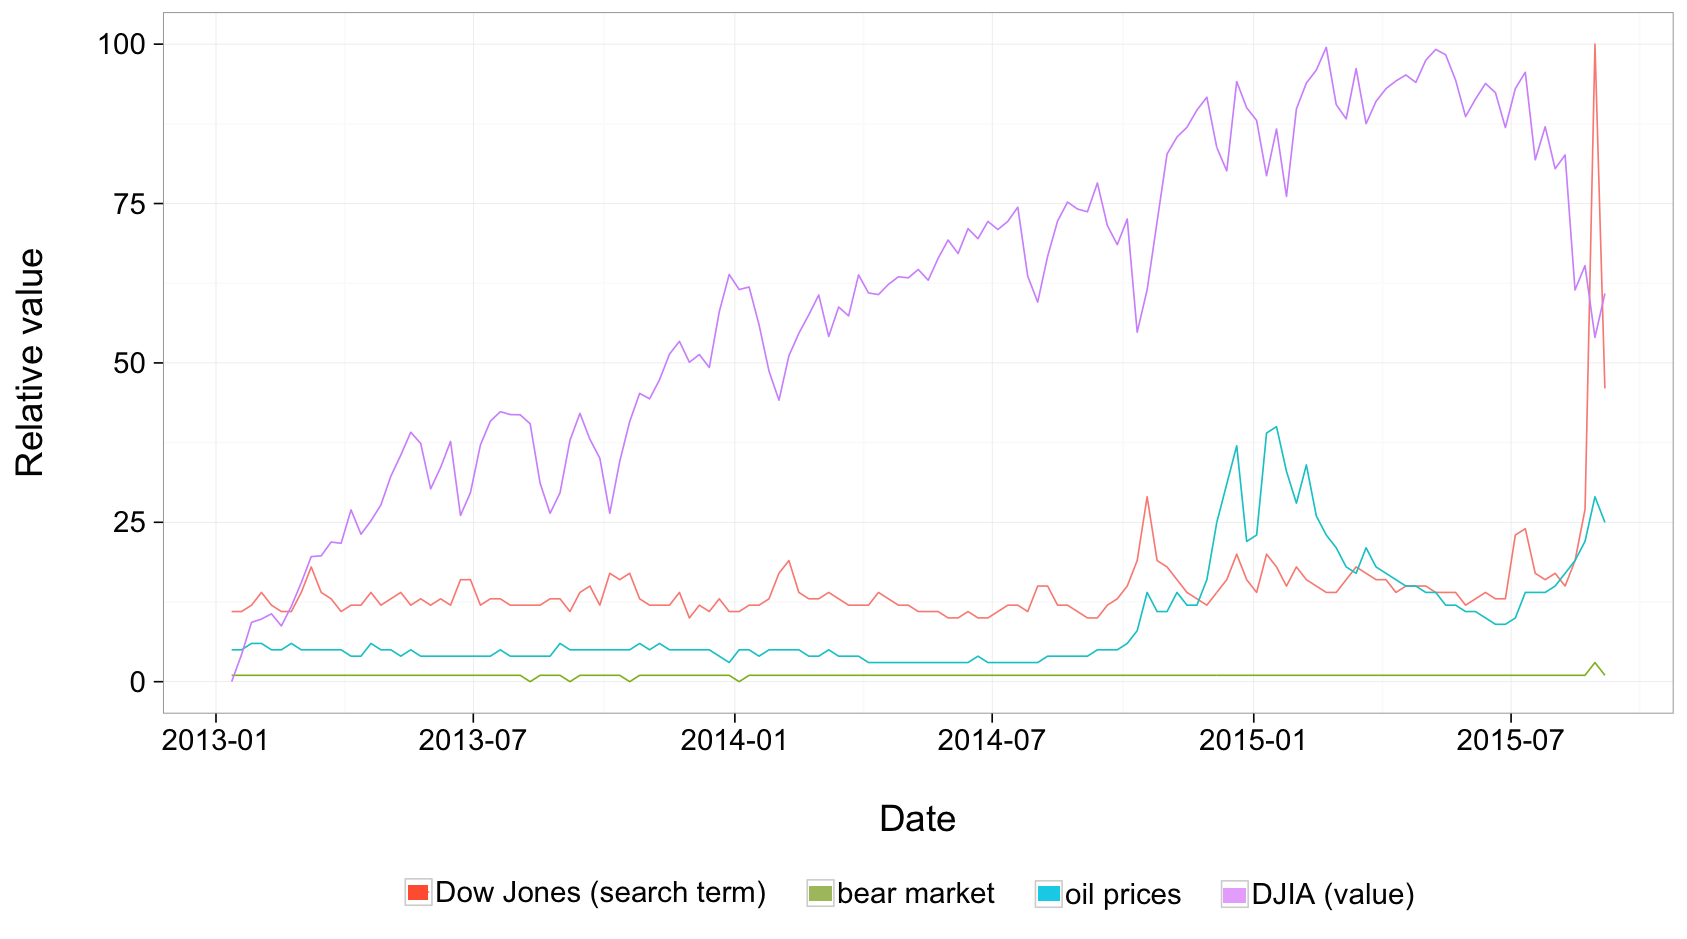
\includegraphics[width=16cm]{/Volumes/Mac OS Drive/Thesis/Source Code/Reporting/nwm_Report/images/google_trends.png}
\caption{\label{fig:gtrends}The relative number of times that the three terms " Dow Jones", "bear market" and "oil prices" were searched for using Google, over the timeline of this study. The price of the Dow Jones Industrial Average (DJIA) is overlaid. The search frequencies are scaled relative to each other, and to lie within the range of zero to one hundred. The DJIA price is scaled independently to the same range.}
\end{figure}

There are two issues that make Google Trends data difficult (but not impossible) to use in the context of this study. The first issue is that the frequency of the data is (at the time of writing) limited to weekly aggregates for timelines longer than three months. This means a method of interpolation would have to be implemented before the data could be combined with daily financial market data over this study's desired time-line of two or more years. Daily data is available for time-lines shorter than three months, which leads nicely on to the second issue. The pre-processing of the data is not transparent; the exact methods used are not published and so any interpretation could perhaps be misleading. The data is clearly normalised, the maximum 'popularity' in each extracted data set being 100 and so \emph{naive} attempts to stitch many three-month data sets together - such as linear combinations - would be in vain, as the final time-line could not be considered homogeneous in scale.

With a different objective in mind, the Google search data does present an interesting case. Hamid and Heiden (\cite{hamid2015forecasting}) were able to show how Google search volumes could be used to increase forecasting accuracy for market phases of relatively high volatility\footnote{This is an interesting direction that could potentially be built upon with the Twitter data accumulated for this study.}. Figure \ref{fig:gtrends} does display a clear correlation between large events in the stock market's price and relative numbers of searches performed on related terms. This is an example of the information that may be extracted from social media data and other meta data. A comparable version to Figure \ref{fig:gtrends} that uses the social media data obtained for this study is provided in Section \texttt{macro-view} (Figure \texttt{fig:tweet-counts-facet}), where similar relationships are highlighted and discussed for the same search terms against the Dow Jones Industrial Average (DJIA).


\subsubsection{Facebook}
\label{sec-1-1-2}
To use Facebook as a source of data, it is necessary to create a special account for software developers (which is free). The downside, however, is that only the publicly available information of your own friends \emph{who also have a developer account} may freely be obtained. This is a large limitation, as it would significantly reduce the amount of data available and narrows down the pool of social media data specifically to a biased subset of users, i.e. data for people who are involved in software development and data mining. This is unfortunately not the target group of this study and so rules out the use of data Facebook.


\subsubsection{Twitter}
\label{sec-1-1-3}
The third option is Twitter, which has been extensively \emph{mined} for its large flow of information (\cite{pak2010twitterMiningEx1}, \cite{bian2012towardsMiningEx2}, \cite{ediger2010massiveMiningEx3}). The following section explains why Twitter is such a popular choice as a source of social media data, justifying its selection for this study. The current best practices of extracting data are then summarised, along with a brief explanation of the procedure defined by this study.


\subsection{Twitter Mining}
\label{sec-1-2}


\subsubsection{Why use Twitter?}
\label{sec-1-2-1}

The social media data used for sentiment analysis (see ChapterX) was sourced exclusively from the online social media platform \href{https://twitter.com/}{Twitter$^{\dag{}}$}. The first post (in Twitter terminology, a \emph{tweet}) was made in March 2006 via short message service (SMS), the entire service running off of a single laptop. In the ensuing months the platform began its ascent to popularity, steadily expanding its user-base after its official launch in summer 2006. Not only individuals, but everyone from news companies and sports teams to artists and presidents use Twitter to update their followers, with the potential to reach anybody with an internet connection.

There are several reasons why Twitter data is an attractive candidate as an explanatory variable in a study such as this one. First and foremost, it is content that is created on a continuous basis with almost no filter\footnote{The only limit imposed on users is the 140-character limit placed on each tweet. \href{https://dev.twitter.com/overview/api/counting-characters}{Twitter's actual definition is slightly more detailed$^{\dag{}}$.}}. In short, users may post their thoughts regarding any topic, at any time, for anyone to read. This makes the data an excellent tool for capturing the sentiments and emotions across extremely large demographics of users, in real time.

According to Twitter's \href{https://about.twitter.com/company}{own website$^{\dag{}}$}, it has approximately 320 million monthly active users, with more than 1 billion unique visits each month to sites where Twitter data is embedded. As a comparison, \href{http://www.internetlivestats.com/google-search-statistics/}{Google was reported$^{\dag{}}$} to facilitate over 100 billion searches every month in 2012. \href{http://newsroom.fb.com/company-info/}{Facebook claims to have 1.59 billion monthly active users$^{\dag{}}$}. Although the Google and Facebook figures are larger than those of Twitter, and so would present larger data sets, the content is not as well suited to sentiment analysis and so the purpose of this study. Acquiring data from Google and Facebook is also a different challenge, with certain disadvantages, as was outlined in Section \ref{soc-data}.


\subsubsection{Requirements for Twitter data \label{criteria}}
\label{sec-1-2-2}

At the time of writing, there are several clear ways in which it is possible to obtain Twitter data, each outlined in Section \ref{twitter-sources}, along with their corresponding benefits and drawbacks. When considering which route to take, it should be kept in mind exactly what kind of analysis will ultimately be performed on the data. The context of this study necessitates that the information obtained fulfils three criteria. Regarding the data of each individual tweet, there are two criteria:

\begin{description}
\item[{Criterion 1:}] each tweet must contain the tweet text

\item[{Criterion 2:}] each tweet must contain a timestamp
\end{description}

The third requirement concerns the population of tweets obtained:

\begin{description}
\item[{Criterion 3:}] the collective corpus of tweets must span a timeline of at least two years
\end{description}

In order to perform sentiment analysis on the Twitter data, it is imperative that the text string is obtained, fulfilling \textbf{Criterion 1}. If only meta-data were to be received, e.g. the creation time and point of origin of a tweet, sentiment analysis would be impossible. \textbf{Criterion 2} ensures that the Twitter data (and therefore the results of the sentiment analysis) can be reliably aggregated into \emph{daily data}. This allows for coherent usage with daily financial market data. Although the timeline specified by \textbf{Criterion 3} may appear somewhat arbitrary (and it is!), a minimum timeline of several years is commonly desired for time-series analysis of financial markets. For discussion as to why this is the case, please refer to the second half of Section \texttt{param-grid}.


\subsubsection{Sources of Twitter data \label{twitter-sources}}
\label{sec-1-2-3}


\paragraph{Twitter API}
\label{sec-1-2-3-1}
Twitter offers an application programme interface (API) to allow programmatic connections to its databases. This is commonly achieved using languages such as Python, JavaScript and R, but can be implemented using any language capable of establishing an API connection.
The service is free, requiring only that users create a developer account, obtaining secure identification methods using a token system. Furthermore, the tweet data is very clean and there are many tools\footnote{The most useful implementation in R is currently the \href{https://cran.r-project.org/web/packages/twitteR/index.html}{\emph{twitteR$^{\dag{}}$}} package, which is a one-stop-shop for cleanly extracting tweets, ready for analysis with common R functions.} already available that parse and display that data.

There are two restrictions placed on the API. The first is to safeguard the Twitter servers from being overrun, namely that each user may make only \href{https://dev.twitter.com/rest/public/rate-limits}{a certain number of requests$^{\dag{}}$} in a given time-frame, which translates into a limit of approximately 10,000 tweets in a fifteen-minute time frame. The second restriction limits the API's reach into the past to approximately seven days. This means that it is impossible to collect and create a time-series of the required length for this study. While it is possible to implement and automate a script to collect tweets at a given frequency\footnote{The author has already implemented such as system, available on request.}, one would have to still wait e.g. two years minus seven days to obtain a time-series that is two years in length. For this reason, the Twitter API methodology was not a feasible option for this study.



\paragraph{Third Party Providers}
\label{sec-1-2-3-2}
It is possible to gain access to the complete Twitter archives, spanning back to Twitter's inception. This is facilitated by a third party company called \href{https://unionmetrics.com/product/echo-twitter-archive-search/}{Union Metrics via their Echo product line$^{\dag{}}$}. There are interactive analytics tools built in to the console, which allow the slicing and drilling of the entire database with visual representations. This is aimed at commercial users needing to make strategic marketing decisions, rather than perform statistical analysis or make quantitative forecasts.

Although the product is extensive and offers many features, it has three potential drawbacks. Firstly it is not a free service; requiring a corporate level monthly subscription. Secondly, the offering is not optimised for independent data analysis, as restrictions on exporting the data would impede full usage of the data within alternative, independent, software packages. Lastly, the fact that a third party is handling the data between it appearing on Twitter and being used in a model adds a \emph{black-box} step that could alter the data, which could produce inconsistencies. All three constraints rule this out as a valid option for this study, with the second constraint being particularly restrictive for parties interested in quantitative forecasting.


\paragraph{Twitter Advanced Search (TAS) \label{TAS}}
\label{sec-1-2-3-3}

The \href{https://twitter.com/search-advanced?lang\%3Den}{Twitter Advanced Search$^{\dag{}}$ (TAS)} web interface allows any user to search for tweets in any time period, displaying tweets that match a given search term. The tweets are displayed in reverse chronological order (the most recent tweet is at the top of the webpage) and each tweet is displayed with its key information. The HTML code being rendered, however, holds additional information, matching all that is available via the API and third party options. There isn't only the tweet text, username and timestamp, but rather a whole host of meta data including e.g. the number of times the tweet has since been \emph{retweeted} (re-posted or shared by another user) or \emph{favourited} (marked as a favourite by another user) and even the longitude-latitude coordinates of the user at the time of posting\footnote{The coordinates accuracy is approximately a 1.5 km radius, which should guarantee some level of privacy.}. Section \ref{html-parsing} goes into more detail about how this data may be located and extracted from the HTML code.

The web interface is free to use, contains the entire Twitter archive and also, being Twitter's \emph{advanced search}, allows for filtering of tweets beyond a date range. For example, the natural language of the tweets (English, Portuguese, etc.) can be used as a filter as well as a longitude-latitude coordinates from which a tweet was posted. Tweets for individual users or containing specific hashtags\footnote{Hashtags provide an unmoderated way to help to link tweets from different users and locales by theme.} can also be selected. This study uses solely the common search function, returning all tweets that contain the user-specified word(s).

The single disadvantage of this approach is that it involves using an interactive interface, i.e. it is not designed to be utilised programmatically. This created significant challenges within the scope of this study, including the development of a customised web-scraper, as shall be explained in the following section.

Before a suitable web-scraper can be outlined, a description of the interface offered by TAS must be given. TAS is a \emph{dynamically loaded} webpage interface to a database, which means that it has access to a great deal of information. When called upon, however, only a small portion of the results are displayed to begin with; the next portion being loaded as soon as the user has scrolled to the bottom of the webpage. This is a common feature implemented by many websites that host data-heavy content, as it enhances the user experience by delivering a \emph{lazy evaluation} or \emph{just in time} approach - data is loaded only at the moment it is required. Other examples are the Google image search results page and a Facebook user's main news feed.


\subsection{Constructing a web-scraper}
\label{sec-1-3}


\subsubsection{What is a web-scraper?}
\label{sec-1-3-1}

To explain this, a good analogy between the internet and an encyclopaedia can be used. Imagine we would like to find all the pages in the encyclopaedia that contain information regarding a topic of intereste, for example "chocolate". We would look in the index for our search term and find all topics involving chocolate to be listed with their page and section numbers. The term given to such a mechanism is \textbf{\href{https://en.wikipedia.org/wiki/Web_crawler}{\emph{web-crawler$^{\dag{}}$}}} and is (simplistically speaking) approximately what search engines such as Google, Yahoo and Bing carry out each time somebody uses their search functions. They look at all the pages in their encyclopaedia and the returned search results are those (web-)pages containing the word "chocolate"\footnote{Web-crawling also includes \emph{how} the search engines obtain their information (i.e. the encyclopaedia) to begin with. An explanation of this does not lie within the scope of this study. \href{http://link.springer.com/article/10.1023/A:1019213109274}{Heydon and Najork (1999)$^{\dag{}}$} provide a good starting point.}. The data in which this study is interested, however, is not the page number, i.e. the internet address of certain information, but rather the contents held at those addresses.

Assuming that the information provided by a web-crawler is already known (in our case the internet address of TAS), using our analogy, we visit the specified page and make a copy of all the information that is stored there. Just as one could write out a copy of any information visible in an encyclopaedia, it is possible to make a copy of all visible information (plus additional background \emph{meta} data) presented on a website. This is because, in order for the website to be displayed in a browser, all the required information must first be transferred (downloaded) to the local device and stored in the form of HTML code, which the browser then interprets and renders. It is then this HTML code that is copied, or \emph{scraped}, leading to the term \textbf{\emph{web-scraper}} \footnote{Also referred to as web harvesting and web data extraction.}.

In order to obtain all required information from TAS, the first major objective of this study was to create a web-scraper that was able to visit the TAS interface, manipulate the webpage and make a copy of the underlying information i.e. the HTML code.


\paragraph{Types of web-scraping}
\label{sec-1-3-1-1}

Web-scraping can be performed in two ways: with a visible browser interface (e.g. what a user sees when using Microsoft Internet Explorer or Google Chrome), or via a \emph{headless browser}. The latter refers to a method whereby a computer connects to a web-address and collects the information held there (the HTML code), but does not render that code in a browser, meaning the user does not see any actual webpages\footnote{\emph{Headless browsing} is a technique often used for debugging purposes, as errors can be detected without visualisation i.e. without rendering the underlying information. This accelerates the process of web-development.}. This method is preferable over the former as it does not require as much computational power and does not consume much working memory on the local device, meaning it can be executed relatively quickly and for a large number of websites. In such a framework it is the connection speed between local device and target that is the limitation. Headless browsers are nevertheless (at the time of writing\footnote{\href{http://stackoverflow.com/questions/34942103/headless-endless-scroll-selenium}{Progress is being made$^{\dag{}}$} in the development of headless browsers for tasks such as scrolling dynamically loaded webpages}) limited to static web-addresses, meaning that the information is held at an address and does not change. However, as was explained in Section \ref{TAS}, TAS has a dynamically loading interface and so requires the former approach, which is described in the following section.


\subsubsection{How does our web-scraper work?}
\label{sec-1-3-2}

To provide the functionality required to manipulate a browser via its graphical user interface (GUI) - as the case is using TAS - a software development tool called \href{http://docs.seleniumhq.org/}{Selenium WebDriver$^{\dag{}}$} was used\footnote{A detailed technical explanation of this step shall not be provided here.}. This facilitated the automation of web-page manipulation. To name several examples, Selenium WebDriver is able to perform actions such as clicking, scrolling and entering text into text-fields - all specified programmatically.

As inputs, TAS takes a search term, any filters that a user adds and a date range. As output, the youngest 20 tweets in the date range are returned, all of which contain the entered search term. Once the user has scrolled to the bottom of the page, the next 10 tweets are loaded. This process continues until the end of the date range is reached, i.e. \hspace{-6pt} once the oldest tweet within the date range has been loaded and displayed. At this point any attempt by the user to keep scrolling will have no effect - no more tweets will be loaded.

The three necessary input for this study are: (1) date range, (2) the search term and (3) a filter to receive only tweets written in English\footnote{Although Twitter includes this as an option within TAS, it is not guaranteed to classify the language with 100\% accuracy.}. These are all able to be specified simply through their inclusion within the target URL\footnote{A Uniform Resource Locator (URL) can contain several elements, but usually essential are a protocol (\emph{http:}) and a host-name \emph{(www.twitter.com)}. More specific locations are then appended as necessary, commonly separated by a forward slash.}. Selenium then enters this URL into the browser's address field and visits that page.

Once the browser has reached the URL and the first 20 tweets resulting from the request specified in the URL have been loaded, a basic process is followed and can be summarised by the following steps:

\begin{enumerate}
\item scroll to the bottom of the page
\item wait long enough for the next 10 tweets to be loaded
\item scroll to the bottom of the page again
\item Repeat steps 2. and 3. until no more tweets load
\end{enumerate}

A programme to automate this process was written in Python, importing the Selenium WebDriver package. A fuller description of the automation process is described by Algorithms \eqref{alg-page-scrape} and \eqref{alg-batch-scrape}, which are defined and discussed in Section \ref{iterative-scraping}.


\paragraph{Stability considerations}
\label{sec-1-3-2-1}

As previously mentioned there are computational constraints to consider when working with a browser. In the case of this task it was the working memory\footnote{Random Access Memory (RAM).} that posed the largest bottleneck. Because the web browser receives, stores and renders the information for all tweets, the amount of memory required increases very quickly. Certain steps can however be taken to reduce this burden, and may be divided into two branches: programmatic and organisational.

In terms of organisation, it was necessary to create batch-processes to perform \emph{scrolling sessions}, which provided control and stability when scrolling downwards over the extremely long dynamically loaded webpage, TAS. It was not possible to scroll to the bottom of the page until tweets for the desired timeline were all loaded, and so a scroll session describes a small segment of this process. Due to the fact that the number of tweets posted that contain a given search term - over any given time-span - cannot be known in advance, the required duration of a scroll session had to be determined heuristically. This duration was determined through a variable defined as the \texttt{scroll.limit}, which tells Selenium how many times to scroll down - pausing for a given time between each scroll to allow TAS to respond and load the next 10 tweets. This process of breaking down the timeline into more manageable segments is named a /batch-process/\footnote{From here on a 'batch' is used synonymously with a 'scroll session'.}.

When the Twitter timeline is being scrolled along, during a single batch, it is helpful to imagine that we are scrolling ever further into the past. Each time the user scrolls downwards and more tweets are loaded, these newly loaded tweets are \emph{older} than the previous tweets.
In order to find a pragmatic value for the \texttt{scroll.limit}, a lot of test-runs were carried out. A sensible value depends on how many tweets a given search term provides - compare the number of tweets obtained for search terms 'interest rates' and 'bull market' in Section \ref{final-output}. It was determined that each date-range would be two weeks in length, and that a \texttt{scroll.limit} of 600 would provide a good compromise between stability and data collection performance. The danger of a longer date range would be that the computer would run out of memory and crash. An insufficient \texttt{scroll.limit} could lead to a scrolling session being ended prematurely, before the last tweet from the date range was loaded.

The greatest gain in performance made through programmatic technique was gained by creating a custom browser profile that the Selenium package then called upon when opening the browser. Within such a profile (depending on the choice of browser used\footnote{Drivers for Mozilla Firefox, Google Chrome and others exist, however \href{https://sites.google.com/a/chromium.org/chromedriver/getting-started}{\emph{ChromeDriver$^{\dag{}}$}} proved itself to be the most reliable when highly customised.}), it is possible to make tweaks such as to prevent images from being downloaded and rendered, which is of course the main culprit of memory allocation. Furthermore, one can provide a chosen identity to present a target address with, which can determine the form of the data a target supplies to a visitor. Presenting oneself, for example, as a 2008 version of a browser could limit the quality of certain meta data that a target sends, with lower quality meaning less information, leading to lower memory requirements.
These techniques were necessary to allow each scrolling session to run as long as possible before significantly eroding performance or possibly crashing, losing all progress.


\subsubsection{Iterative web-scraping \label{iterative-scraping}}
\label{sec-1-3-3}

Each target URL was composed manually for each two-week date range. It including start and end dates for date range, a filter to return only English language tweets, plus one search term. [An example URL in appendix?]. This URL was then passed to Selenium, a browser was launched and the scrolling session commenced. The \texttt{scroll.limit} was set equal to 600 and a \texttt{scroll.count} variable was initialised to zero. Algorithm \eqref{alg-page-scrape} describes the iterative process performed by the web scraper for each scroll session defined.

\vspace{5mm}

\begin{algorithm}[H]
  \caption{Iterative web-scraping algorithm for a dynamically loading website}
  \label{alg-page-scrape}
  \SetKw{Return}{return} %% Custom keyword

  \BlankLine
  \BlankLine
  \KwIn{target URL, scroll.count, scroll.limit}
  \KwOut{HTML code}
  \BlankLine
  
  \Repeat{scroll.count = scroll.limit} {
    scroll to bottom of page\;
    \eIf(\tcc*[f]{waiting time purely heuristic}){current position at end of page} {
      wait 3 seconds for next tweets to load\; 
      current position $\leftarrow$ new position\;
    } 
    {
      scroll to bottom of page\;
    }
    increment scroll.count
  }
  \BlankLine
  \BlankLine
  \Return{HTML source code} \tcc*[f]{saved to disk as .txt file}
\end{algorithm}

\vspace{5mm}

In the last stage of Algorithm \eqref{alg-page-scrape}, \texttt{scroll.count} has reached 600 and it is assumed that the last tweet within the date range has been loaded before the HTML code is copied and saved.
Algorithm \eqref{alg-batch-scrape} depicts how Algorithm \eqref{alg-page-scrape} is extrapolated into a batch process that to obtain tweets covering the entire time-span - each scroll session covering the specified two-week date range. For this second algorithm, several further variables are defined. Given we have a list of search terms for which we would like to collect tweets, the variable \texttt{search.term} represents which single search time we are currently considering. The \texttt{time-span} is the total timeline of interest, previously stated to be several years or more. According to the iterative process outline above, this is then decomposed into smaller batches, where \texttt{time-span-segment} represents a two-week date range.

\vspace{5mm}

\begin{algorithm}[H]
  \caption{Batch-process to recursively scrape over desired time-span for each search term}
  \label{alg-batch-scrape}

  \BlankLine
  \BlankLine

  \KwIn{time-span, search.terms}
  \KwOut{Aggregated HTML code}
  \BlankLine

  \ForEach(\tcc*[f]{each search.term amounts}){search.term} {
    \ForEach(\tcc*[f]{to 70 time-span-segments}){time-span-segment in time-span} {
      execute Algorithm 1\;
    }
  }   
\end{algorithm}

\vspace{5mm}

Once both Algorithms \eqref{alg-page-scrape} and \eqref{alg-batch-scrape} had completed, the HTML code for each search term over the entire desired timeline was obtained. This is however not a usable format, and required processing in order to extract the required data as set out by Criteria 1-3 in Section \ref{criteria}. The following section outlines how this was achieved.


\subsubsection{Parsing the HTML code \label{html-parsing}}
\label{sec-1-3-4}

HTML\footnote{\href{https://en.wikipedia.org/wiki/HTML}{Hyper Text Markup Language$^{\dag{}}$.}} is a feature-rich language that drives the majority of web-based applications. Having said that, all that must be known for the scope of this study is that HTML provides the structure of a webpage, holding all the elements such as text and images in place - simplifying the task of identifying and locating elements for interpreters such as web-browsers. It is this particular feature that allows the HTML code to be parsed, retrieving specific information.

There is a large online community that provides a great deal of expertise and support in this area. This is essential because, although there are \href{http://www.w3.org/TR/html51/}{agreed standards$^{\dag{}}$}, the way people create their webpages changes almost on a daily basis alongside the development and implementation of new features and platforms. Here we briefly describe the HTML language and the possible ways of extracting information from its raw form.


\paragraph{HTML parsing methods}
\label{sec-1-3-4-1}

All information contained within HTML is held within an \emph{element tree}, with all similar items held at the same levels, or branches. There are currently two established and proven methods to scale and search this element tree and extract information, namely the Extensible Markup Language Paths (XPath) and Cascading Style Sheets (CSS) methodologies\footnote{\href{http://elementalselenium.com/tips/32-xpath-vs-css}{A side-by-side comparison$^{\dag{}}$} shows them to perform similarly. \href{http://saucelabs.com/resources/selenium/css-selectors}{One can also translate between them$^{\dag{}}$.}}. A brief history of their development and usage, as well as the tools that were created to exploit them is given by \cite{krijnen:automated}.

CSS offers a very quick way way to locate elements within the element tree, due to a reliance on extremely precise descriptions that are used for each element. As the name implies, the CSS search route \emph{cascades} down the tree, and it can only move in this direction. XPaths provide a more robust method of HTML parsing, being able to scale both up and down the element tree, on top of using higher abstractions of element locations. This added robustness and reliability comes at a price, namely the speed of operation. It suffices to say that there is a slight speed to stability trade-off to be made when selecting which method to use. As the Twitter interface is regularly updated, stability was valued over speed (the difference being several hours, when parsing all scraped HTML code). The XPath method was therefore chosen as the preferred method.


\paragraph{The extracted data}
\label{sec-1-3-4-2}

In addition to the three criteria listed in Section \ref{criteria}, there was further useful information to be salvaged from the raw HTML code that scraping produced. The data useful for this study, and was indeed extracted, is summarised in Table \ref{table:twitter-data-usage}. The \emph{Description} column describes the data available for each tweet, whereas the \emph{Usage} column outlines how it was ultimately used within the modelling.

\vspace{3mm}

\begin{table}[htb]
\centering
\begin{tabular}{lllll}
\textbf{Data} &  & \textbf{Description} &  & \textbf{Usage}\\
 &  &  &  & \\
\hline
 &  &  &  & \\
timestamp &  & A millisecond accurate timestamp &  & The calendar day\\
tweet-ID &  & A unique identifier &  & Remove any duplicates\\
tweet text &  & The text string (max. 140 characters) &  & Sentiment analysis\\
times retweeted &  & Number of times a tweet was retweeted &  & As variable and weighting factor$^{\text{*}}$\\
times favourites &  & Number of times a tweet was favourited &  & As variable and weighting factor$^{\text{*}}$\\
 &  &  &  & \\
\end{tabular}\caption{\label{table:twitter-data-usage}Summary of Twitter data usage}

\end{table}

\mbox{*} This is explained in detail in Section \texttt{weighting-sentiment}. 

\vspace{5mm}

The actual output of all the scraping and parsing efforts up until this point was one text file for each of the two-week date ranges. In each file there was one row of data for each individual tweet, containing the information listed in Table \ref{table:twitter-data-usage}.

When working at the intersection of several languages (here primarily between HTML, Python and R), there are often data conversion issues. This was nowhere more a problem than with the extracted Twitter data. Certain characters are no-longer legible once taken away from a web-browsing context, meaning that a large amount of post-processing was necessary in order to leave the data in a state that the sentiment analysis models were able to interpret. An example of the \emph{cleaning process} that each individual tweet must pass through before being passed to the sentiment analysis models is shown in the following below in Section \ref{cleaning-tweets}.


\subsubsection{Post-processing tweet text \label{cleaning-tweets}}
\label{sec-1-3-5}

As touched upon in the previous section, the extracted Twitter data still required cleaning before sentiment analysis could be performed. This was a crucial procedure for two reasons. Firstly because the sentiment analysis models are written in yet further collections of languages such as Java and Perl, meaning, for consistencies sake, that the input to all models (i.e. the tweet text data) should be in as pure a form as possible. Secondly, the models need to make sense of the input data and to do this, they have pre-defined dictionaries and comprehensions of grammar. While the model creators did keep modern language use, abbreviations and slang in mind (to name just a few factors), the models will not be able to make sense out of non-sense. \newline Two main steps were performed:

\begin{enumerate}
\item Removal of all operating system dependent characters, for example Windows carriage returns: \texttt{\textasciicircum{}M}

\item Selective removal of many non-standard characters according to an ASCII framework\footnote{A system by which all characters can be \href{http://www.asciitable.com/}{represented$^{\dag{}}$} in a uniform manner across all platforms and for all audiences. This means both humans and machines must have an unambiguous translatory method.}
\end{enumerate}

Fortunately there is a relively rapid method for performing the first point. That is namely to run all text files through a UNIX command named \texttt{dos2unix} whilst on a unix based system. After performing this, there are no longer artefacts stemming from the operating system used for the scraping process.

The second point is rather more complicated and best illustrated with a short example. The following text string is taken from the tweet data directly after being extracted from the HTML element tree:

\begin{verbatim}
  """I wonder what people think about the Dow Jones Industrial Average ""Death Cross""
  now? :)^M #trendfollowing pic.twitter.com/nnyXLMlShA^M"""
\end{verbatim}

Inspecting this raw tweet text, it is clear that there are non-sensical parts. For example, all being contained in three speech-marks, the two carriage returns, and a random collection of letters at the end of in the URL. One interesting part, however is the \emph{smiley}. This is something that is not a standard word contained in a dictionary, however many of the sentiment analysis models do contain a lexicon of such modern additions to text, predominant in social media data. It is for this reason that step two was labelled as the \emph{selective} of certain elements.

This step was performed with R and is not explained in depth here. In one sentence: regular expressions using the Perl \href{http://www.pcre.org/}{PRCE engine$^{\dag{}}$} were created, utilising hexidecimal character definitions to identify and remove specified ranges of ASCII characters. An annoted version of the function that was defined to achieve this for all tweets can be found in Appendix \texttt{XX}.
The output is a text string that is interpretable by the sentiment analysis models:

\begin{verbatim}
  I wonder what people think about the Dow Jones Industrial Average Death Cross now?
  :) trendfollowing
\end{verbatim}


\subsubsection{Final output for sentiment analysis \label{final-output}}
\label{sec-1-3-6}

Up to this point in the workflow, Twitter data has successfully been scraped from TAS, the results HTML code has been parsed and every single tweet has been cleaned, in a form ready to be used for sentiment analysis. This path has been visualised with a flowchart, found in Appendix \texttt{XX}. Some summary information of the Twitter data can now be presented:

\vspace{3mm}


\begin{center}
\begin{tabular}{llll}
 & \textbf{Number of search terms:} &  & 13\\
 &  &  & \\
 & \textbf{Total timeline:} &  & 982 days (695 weekdays)\\
 &  &  & \\
 & \textbf{Date range:} &  & $14^{th}$ January 2013 $\rightarrow$ $11^{th}$ September 2015\footnotemark\\
 &  &  & \\
 & \textbf{Total tweets obtained:} &  & $2,350,217$\\
 &  &  & \\
\end{tabular}
\end{center}\footnotetext[20]{This date range is the one ultimately used; however, tweets were obtained over a slightly longer period, which is reflected in Table \ref{tab.tweet-breakdown}.}


\vspace{3mm}

\begin{table}[htb]
\centering
\begin{tabular}{lrlclr}
\textbf{Search term} & \textbf{Total tweets} &  & \textbf{Days} &  & \textbf{Time-span coverage}\\
 &  &  & (max. 982) &  & (\% of 982 days)\\
\hline
 &  &  &  &  & \\
bear market & 47,924 &  & 963 &  & 98.1\\
bull market & 74,937 &  & 965 &  & 98.3\\
dow jones & 250,112 &  & 982 &  & 100.0\\
dow SPDR & 1,628 &  & 700 &  & 71.3\\
dow wallstreet & 26,395 &  & 921 &  & 93.8\\
federal reserve & 378,970 &  & 904 &  & 92.1\\
financial crisis & 261,500 &  & 922 &  & 93.9\\
goldman sachs & 289,485 &  & 909 &  & 92.6\\
interest rates & 396,765 &  & 857 &  & 87.3\\
market volatility & 60,858 &  & 970 &  & 98.8\\
obama economy & 202,654 &  & 908 &  & 92.5\\
oil prices & 219,766 &  & 785 &  & 79.9\\
stock prices & 139,223 &  & 982 &  & 100.0\\
 &  &  &  &  & \\
\textbf{Total/max./avg.} & 2,350,217 &  & 982 &  & 100.0\\
 &  &  &  &  & \\
\end{tabular}\caption{\label{tab.tweet-breakdown}A breakdown of the total number of tweets extracted by search term, including the number and percentage of total days covered across the entire timeline.}

\end{table}

Looking at Table \ref{tab.tweet-breakdown}, we notice that the search terms with lower time-span coverage are those that are very market driven (e.g. "dow SPDR" and "oil prices") and so are likely to not be talked about very frequently at weekends. Using the number of tweets to weight each of the search terms, the weighted average time-span coverage is 92.2 \%. Indeed, as soon as weekends are removed from the equation (a necessary step in the modelling to combine Twitter data with financial market data), the time-span coverage jumps to 99.3 \%, which is equivalent to saying that the percentage of missing sentiment data was 0.7 \% at the point of being combined with financial market data. Imputation was subsequently performed, as described in Section \texttt{imputation}.

\pagebreak


\subsection{Function to clean tweets using hexidecimal definitions}
\label{sec-1-4}

\begin{listing}[H]
\begin{minted}[frame=lines,linenos]{r}
##  Hex codes: http://www.asciitable.com/
##  The characters each line removes are displayed
tweet.cleaner <- function(x) {

    gsub("&amp;", "&", x) %>%
        gsub("[^\\x{20}-\\x{7F}]", "", ., perl = TRUE) %>%  # Leaves ASCII characters
                                                  # Removes:
        gsub("\\x{22}*", "", ., perl = TRUE) %>%  # "        
        gsub("\\x{23}*", "", ., perl = TRUE) %>%  # #           
        gsub("\\x{24}*", "", ., perl = TRUE) %>%  # $
        gsub("\\x{25}*", "", ., perl = TRUE) %>%  # %
        gsub("^\\x{27}", "", ., perl = TRUE) %>%  # '                
        gsub("\\.{2,}", " ", ., perl = TRUE) %>%  # two or more .
        gsub("\\x{2A}*", "", ., perl = TRUE) %>%  # *
        gsub("\\x{5B}*", "", ., perl = TRUE) %>%  # [
        gsub("\\x{5D}*", "", ., perl = TRUE) %>%  # ]
        gsub("\\x{5F}*", "", ., perl = TRUE) %>%  # _
        gsub("\\x{60}*", "", ., perl = TRUE) %>%  # `
        gsub("[\\x{7B}-\\x{7F}]", "", ., perl = TRUE) %>%  # 5 characters: { | } ~ DEL
        gsub("http\\S+\\s*", "", .) %>%  # remove URLs
        gsub("^\\.?", "", .) %>%  # Remove any . at beginning of string
        stripWhitespace() %>%
        gsub("^ ", "", .) %>%
        gsub(" $", "", .)
}
\end{minted}
\caption{\label{mycode:tweet-cleaner}The function used to remove selective characters from raw tweet data. \textbf{Note:} the \emph{Perl} regular expression engine must be specified}
\end{listing}
% Emacs 24.5.1 (Org mode 8.2.10)
\end{document}